\section{Anonymous Live-CDs f�r JonDo und Tor}
Es gibt einige Projekte, die eine Live-CD bereitstellen. Bei der Nutzung einer Live-CD erh�lt man ein sinnvoll vorkonfiguriertes und garantiert sauberes System ohne Trojaner. Da man keine Updates einspielen kann, sollte man regelm��ig eine aktuelle Version des ISO-Images von der Webseite herunter laden.

\begin{description}
 \item[JonDo Live-CD/DVD] basiert auf Debian GNU/Linux und bietet JonDonym, Tor und Mixmaster als Anonymisierungsdienste. Mit JonDoBrowser ist ein sicherer Browser installiert. Der E-Mail Client Icedove ist f�r anonyme Nutzung vorbereitet. Au�erdem sind Pidgin, Jitsi, Skype, der Parole Media Player und weitere Anwendungen enthalten.\\

 Die Live-CD/DVD gibt es mit deutscher Lokalisierung. Es ist ein Hybrid-ISO und kann sowohl mit Intel i686 als auch mit AMD64 Computern genutzt werden. Beim Booten werden MAC-Adressen der Netzwerk�schnittstellen gefakt, um eine hohe Anonymit�t in Internetcafes u.�. zu erm�glichen. \\

 Download: \href{https://www.anonym-surfen.de/jondo-live-cd.html}{https://www.anonym-surfen.de/jondo-live-cd.html}

 \item[TAILS] \textit{The Amnesic Incognito Live System} ist die offizielle Live-CD von Torproject.org. Der gesamte Datenverkehr ins Internet wird in der Standardkonfiguration durch Tor geschickt. Die Live-CD wird aktiv weiterentwickelt und bietet eine sehr hohe Qualit�t hinsichtlich Sicherheit. \\

 TAILS bietet die Anonymisierungsdienste Tor und I2P. Diese Live-CD kann nur mit Intel i686 Computern genutzt werden. \\

 Download: \href{https://tails.boum.org/}{https://tails.boum.org/}

 \item[Polippix] ist eine Tor-Live-CD von der IT-Political Association of Denmark basierend auf Linux. Die letzte Version ist vom Juli 2010, also etwas veraltet. Es gibt eine deutsche Anleitung vom AK Vorrat.\\

 Download: \href{http://polippix.org/}{http://polippix.org}

 \item[Privatix] von Markus Mandalka bietet ebenfalls Tor als Anonymisierungsdienst. Als Internet Anwendung ist lediglich Icewaesel (die Debian-Version von Firefox) mit TorButton + Polipo vorkonfiguriert. Im Gegensatz zu TAILS und Polippix wird nicht der gesamte Datenverkehr durch Tor gejagt.\\

 Ein besonderes Feature von Privatix ist der Installations-Wizard f�r USB-Sticks. Der Wizard verschl�sselt das System bei der Installation vollst�ndig und erstellt ein schreibbares System (im Gegensatz zu UNetbootin). Privatix wird relativ selten aktualisiert, in der Regel nur mit einem neuen Debian Release. Deshalb empfehlen wir die Installation auf einem USB-Stick und regelm��iges Einspielen der Security-Updates.\\

 Download: \href{http://www.mandalka.name/privatix/}{http://www.mandalka.name/privatix/}

\item[Ubuntu Privacy Remix] soll an dieser Stelle auch erw�hnt werden. Es ist eine Live-CD ganz ohne Netzwerkverbindungen. Diese Live-CD erm�glicht ein sicheres Bearbeiten von Dokumenten in einer garantiert sauberen Umgebung, ein L�sung f�r spezielle F�lle.
 \end{description}

Alle Live-CDs k�nnen als ISO-Image auf einen CD-Rohling gebrannt oder auch mit einem USB-Stick genutzt werden. Die Nutzung des USB-Sticks als Boot-Medium bringt einen deutlichen Geschwindigkeitsvorteil. Mit dem Tool \textbf{UNetbootin} kann man ein ISO-Image problemlos auf einen USB-Stick ``brennen``. F�r Windows und MacOS ist die Software von der Projektseite \href{http://unetbootin.sourceforge.net/}{http://unetbootin.sourceforge.net} herunter zu laden und zu installieren, Linuxer finden ein passendes Paket in den Repositories der Distribution und k�nnen es mit dem Paketmanager installieren.\\

\begin{figure}[htb]
\begin{center}
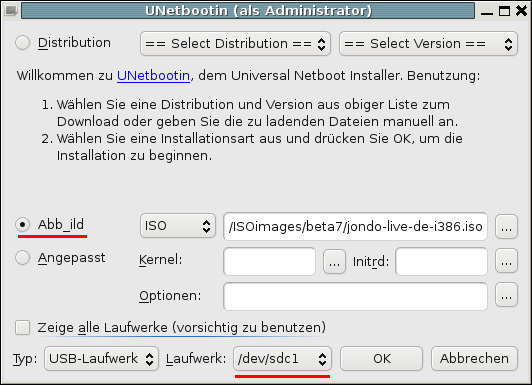
\includegraphics[scale=0.7]{../screenshots/unetbootin1.png}
\caption{UNetbootin GUI}
\end{center}
\end{figure}

Nach dem Start von UNetbootin als Administrator oder root w�hlt man das ISO-Image und den USB-Stick als Ziel. Nach einem Klick auf Ok wird ein bootf�higer USB-Stick erstellt - fertig.\\

Mit UNetbootin ''gebrannte'' USB-Sticks werden beim Booten als read-only eingebunden! Wie bei einer Live-CD gehen alle �nderungen bei einem Reboot verloren. Der Vorteil liegt vor allem in einer h�heren Geschwindigkeit.\\

Au�erdem k�nnen zus�tzliche Daten auf dem Stick gespeichert werden (Lesezeichen, OpenPGP-Schl�ssel, JonDonym Premium Accounts...). Diese zus�tzlichen Daten findet man nach dem Booten des Live-Systems im Verzeichnis \textit{/live/image}.